\documentclass[10pt]{article}
\usepackage{tmlr}            % anonymous submission mode; use \usepackage[preprint]{tmlr} to show authors
\usepackage{amsmath,amssymb}
\usepackage{graphicx}
\usepackage{booktabs}
\usepackage{multirow}
\usepackage{url}
\usepackage{hyperref}
\usepackage{tikz}
\usetikzlibrary{arrows.meta,positioning}
\graphicspath{{figs/}}
\newcommand{\cell}{0.5\,m}
\newif\ifreview \ifdefined\REVIEWMODE \reviewtrue \fi
\newcommand{\J}[1]{\ifreview\textcolor{red}{\textbf{[J#1]}}\,\fi}   % author-judgement markers, shown only in main_review.pdf (see AUTHOR_REVIEW.md)
\newcommand{\pmsd}[2]{#1\,{\scriptsize$\pm$\,#2}}

\title{When Do Echoes Help? Learned Echolocation for Exploring Unseen Buildings\\ in a Sample-Accurate Acoustic Simulator}

\author{\name Anonymous authors \\ \addr Paper under double-blind review}

\begin{document}
\maketitle
{\renewcommand{\thefootnote}{}\footnotetext{Disclosure required by TMLR: a large language model (an AI coding assistant) was used to write the software and to draft the text of this submission under the authors' direction; details are given in the statement ``Use of AI assistance'' before the references.}}

\begin{abstract}
Bats and some blind humans find their way by emitting a sound and listening to its echoes. We ask when a simulated agent trained with reinforcement learning benefits from doing the same, and in what form the echoes should be presented to it.
We first make an existing engine usable for this question. Steam Audio 4.8.1, a widely used ray-traced room-acoustics library, stores reflected energy in 10\,ms bins and fills each bin with noise, so a wall 1\,m away and a wall 2.5\,m away produce the same impulse response. We patch its core to use one bin per audio sample and to emit one impulse per arrival; a reflection from a single wall then starts within one sample (21\,$\mu$s at 48\,kHz) of the image-source prediction, and 26 of 26 analytic checks pass (speed of sound fitted from arrivals: 340.01\,m/s against the engine's 340\,m/s).
We connect the patched engine to Habitat-sim and train recurrent PPO agents that click once per step in complete darkness. On the Replica dataset (14 training buildings, 4 held-out buildings, 3 seeds per agent, 2 million steps each) we find:
\J{1}(i) when a goal vector is supplied, echoes do not improve navigation success in held-out buildings (0.38 with echoes, 0.39 without);
(ii) when the agent must explore without any goal, echoes help substantially: an agent that receives a range-by-direction ``sonar image'' computed from the first-order Ambisonic echo response covers \pmsd{37.0}{1.5} cells of \cell{} in 300 steps, against \pmsd{24.5}{3.9} for a blind agent with a bump sensor and 28.0 for a scripted bump-and-turn explorer, with fewer collisions than either;
(iii) the same echoes presented as binaural spectrograms from three head orientations yield only \pmsd{26.6}{3.3} cells at 2.7 times the simulation cost;
(iv) when the echo carries distance but no direction, agents that choose where to aim each click do not cover more ground than a scripted sweep, but collide least of all agents (\pmsd{15.4}{2.0} collisions per episode) and one of three seeds learns to stay silent on 62\% of steps;
(v) decoders trained on the agents' recurrent states recover which nearby floor cells the agent has already visited in held-out buildings (AUROC 0.76--0.83), and this path memory is strongest in the blind agents, while agents that hear the room hold local geometry in their current observation rather than in memory;
(vi) erasing the recurrent memory every 20 steps reduces the blind agents' coverage by 15\% and leaves the echo agents' coverage unchanged, and erasing it at every step multiplies the echo agents' collisions by 3 to 6 while they still cover 70--100\% of their usual area.
All code, the simulator patch, raw evaluation logs and figure scripts are released.
\end{abstract}

% ======================================================================================================
\section{Introduction}

A click reflected from a wall returns after $2d/c$ seconds, where $d$ is the distance to the wall and $c$ the speed of sound: 5.9\,ms for a wall at 1\,m. Echolocating bats use this delay, together with the direction from which the echo arrives, to fly through clutter in darkness \citep{griffin1958listening,moss2010probing}, and some blind people use tongue clicks in the same way \citep{thaler2016echolocation}. An embodied agent that could do this would have a sense that works without light and needs only a loudspeaker and a few microphones.

Research on learned audio navigation has concentrated on a different problem: reaching a \emph{sounding goal}, usually with vision available \citep{chen2020soundspaces,gan2020look}. Work on echoes has mostly treated them as a supervisory signal for visual representations \citep{gao2020visualechoes} or as input for predicting depth maps \citep{christensen2020batvision}. \J{2}Whether an agent that acts on nothing but the echoes of its own clicks benefits from them, and which properties of the echo signal matter, has not been tested in a controlled way across unseen buildings and random seeds. This paper does that.

\J{3}Such a study needs a simulator in which the arrival time of each echo is correct to well under a millisecond, because 1\,ms corresponds to 17\,cm of range. We found that Steam Audio \citep{steamaudio}, a ray-traced acoustics engine that is open source, fast and actively maintained, does not provide this in its shipped form: it accumulates reflected energy in bins of 10\,ms (3.4\,m of path length) and reconstructs the impulse response by filling each bin with band-limited noise. Section~\ref{sec:sim} describes a small patch that removes this limit and its validation against analytic acoustics.

\paragraph{Contributions.}
\begin{enumerate}
\item \textbf{A sample-accurate, validated echo simulator.} A 172-line patch to the Steam Audio 4.8.1 core (per-sample energy bins and a deterministic ``sparse'' reconstruction, both switched by environment variables), \J{26}three fixes for defects in the upstream code, and a validation suite of 26 analytic checks on a single wall plus 7 checks in a shoebox room, all of which pass. We also document one physical deviation of the engine that the patch does not remove: specular reflection energy is too low by a factor $\cos\theta$ at incidence angle $\theta$ (Section~\ref{sec:deviations}).
\item \textbf{An environment for echo-based embodied learning.} A Gym environment that takes scene geometry, navigation mesh and agent motion from Habitat-sim \citep{savva2019habitat} and computes the acoustics of every step with the patched engine on the same triangle mesh. It provides three echo observations of decreasing richness: binaural spectrograms from several head orientations, a range$\times$azimuth \emph{sonar image} obtained from the Ambisonic intensity vector of each arrival, and a direction-free \emph{range profile} combined with a steerable click beam.
\item \textbf{A controlled study with three seeds per configuration on held-out buildings}, comprising four experiments: a comparison of echo representations for exploration (Experiment~1), a test of learned click aiming when the beam is the only source of direction (Experiment~2), a probe of what the agents' recurrent memory encodes (Experiment~3), and a causal test in which that memory is erased during an episode (Experiment~4). We also report, clearly marked as single-seed, the preliminary runs that shaped the design, including a negative result for goal-directed navigation.
\end{enumerate}

\paragraph{\J{4}Summary of findings.} Echoes did not help our agents reach a goal whose direction and distance they were told at every step; a blind agent with a bump sensor did as well. Echoes helped when there was no goal vector and the agent had to cover unknown floor area: the sonar-image agent covered 51\% more cells than the blind agent with 15\% fewer collisions (Table~\ref{tab:exp1}). The representation mattered more than the amount of acoustic simulation: three binaural spectrograms per step were no better than blindness, one sonar image per step was clearly better. Giving the agent control over the click direction changed its behaviour (it became the most cautious agent and sometimes stopped clicking) but did not increase coverage. Finally, all agents carried a decodable record of their own recent path in memory, and the agents that could not sense walls relied on it most: erasing memory older than 20 steps reduced coverage only for the blind agents (Table~\ref{tab:wipe}).

% ======================================================================================================
\section{Related work}

\paragraph{Audio in embodied AI.} SoundSpaces \citep{chen2020soundspaces} introduced audio-goal navigation with precomputed room impulse responses on a discrete grid of Replica \citep{straub2019replica} and Matterport3D \citep{chang2017matterport3d} scenes; SoundSpaces~2.0 \citep{chen2022soundspaces2} added continuous rendering with a bidirectional path tracer. \citet{gan2020look} studied a similar task. Follow-up work added waypoints and acoustic memory \citep{chen2021waypoints}. In all of these the agent listens to an external source; the agent in our study is its own source. Our environment reuses the SoundSpaces action space and the 1\,s source clips for the audio-goal sanity check, but computes acoustics with a different engine at every step.

\paragraph{Echoes as a learning signal.} VisualEchoes \citep{gao2020visualechoes} uses simulated echoes to pretrain image encoders; BatVision \citep{christensen2020batvision} predicts depth images from recorded binaural chirp echoes; \citet{purushwalkam2021audio} reconstruct floor plans from audio and vision. Robotic work has built bat-like ultrasonic platforms that map and navigate with hand-designed processing \citep{eliakim2018robat}. \J{5}We are not aware of a study that trains navigation or exploration policies on self-generated echoes alone and evaluates them on held-out buildings with multiple seeds.

\paragraph{Exploration and memory in navigation agents.} Coverage rewards for learned exploration follow \citet{chen2019learning} and \citet{chaplot2020learning}. The auxiliary loss we use is in the spirit of \citet{mirowski2017learning} and \citet{jaderberg2017reinforcement}. \J{6}Our probing experiment follows the linear-probe methodology of \citet{alain2017understanding} and is closest to \citet{wijmans2023emergence}, who showed that blind point-goal agents with only egomotion input build map-like representations. We extend that finding to exploration agents with acoustic and bump sensing and compare memory content across sensors.

\paragraph{Acoustic simulation and spatial audio analysis.} The image-source model \citep{allen1979image} gives exact early reflections in a shoebox room and is our reference for validation. The direction estimate we use for the sonar image is the acoustic intensity vector of a first-order Ambisonic signal, as used in spatial impulse response rendering \citep{merimaa2005spatial} and directional audio coding \citep{pulkki2007spatial}. Steam Audio traces rays with its own tracer or with Embree \citep{wald2014embree}.

% ======================================================================================================
\section{A sample-accurate echo simulator}
\label{sec:sim}

\subsection{What Steam Audio computes}
We established the following from the Steam Audio 4.8.1 source code and confirmed each item by measurement with a C program that places one source, one listener and one planar wall in an otherwise empty scene (Appendix~\ref{app:validation}).

Reflections are traced from the listener. At each surface hit the engine adds the irradiance arriving from the source, $1/(4\pi d^2)$ at source distance $d$, multiplied by a reflectance: a specular lobe $\frac{n+2}{8\pi}(\mathbf h\!\cdot\!\mathbf N)^n$ with $n=100$ weighted by $(1-s)$, plus a Lambertian term $\frac{s}{\pi}\cos\theta_i$, where $s$ is the material's scattering coefficient, $\mathbf h$ the half vector and $\mathbf N$ the surface normal; the result is multiplied by $(1-\alpha_b)$ for absorption $\alpha_b$ in each of three frequency bands (below 800\,Hz, 800\,Hz--8\,kHz, above 8\,kHz). The speed of sound is 340\,m/s. Energy is accumulated in a histogram over time, band and spherical-harmonic channel (ACN order, N3D normalisation). Time zero of the histogram is the arrival of the direct sound, so a reflection of path length $r_\text{refl}$ appears at $(r_\text{refl}-r_\text{direct})/c$. Air absorption multiplies energy by $e^{-k_b d}$ with $k_b = 0.0002,\,0.0017,\,0.0182$ per metre. Triangles reflect from both sides. There is no diffraction and no phase change on reflection.

\subsection{The problem: 10\,ms bins filled with noise}
The histogram bins are 10\,ms long. In 10\,ms sound travels 3.4\,m, so all surfaces within 1.7\,m of range fall into the same bin. To turn the histogram into an impulse response the engine multiplies a fixed sequence of uniform noise in $[-1,1]$ by a linear ramp between the square roots of consecutive bin energies and band-limits it. Figure~\ref{fig:ir}a shows the result for one wall: the echo, which should be a single arrival at 12.72\,ms, is a burst of noise extending from 10 to 30\,ms. The total energy and the coarse timing are right (25 of 25 checks on the stock library pass once the binning is taken into account), but an agent cannot measure range from it.

\begin{figure}[t]
\centering
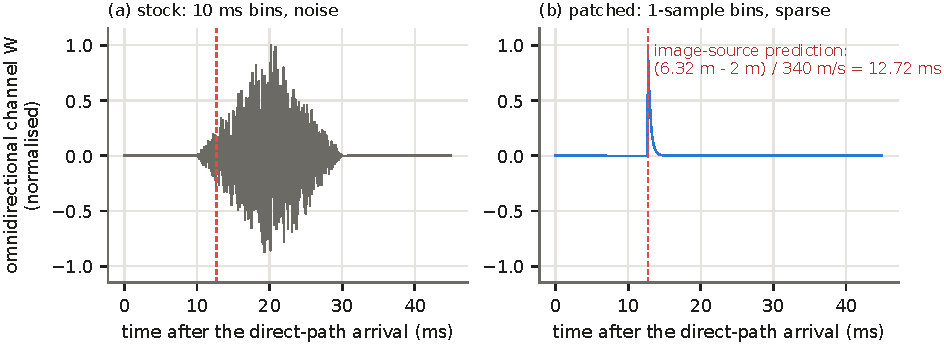
\includegraphics[width=0.95\linewidth]{ir_stock_vs_patched.pdf}
\caption{Impulse response (omnidirectional channel, 48\,kHz) for a source 2\,m from the listener and a fully reflecting wall 3\,m to the side, so that the image source is 6.32\,m away and the reflection should arrive 12.72\,ms after the direct sound (dashed line). (a) Stock Steam Audio 4.8.1. (b) The patched core used in this paper; the short tail after the onset is the engine's glossy ($n=100$) specular lobe.}
\label{fig:ir}
\end{figure}

\subsection{The patch}
\label{sec:patch}
The patch changes 11 files (172 lines added, 13 removed). With no environment variable set the library behaves exactly as shipped.
\begin{itemize}
\item \textbf{Bin duration.} The constant 0.01\,s becomes a value read from \texttt{STEAMAUDIO\_BIN\_DURATION}. We set it to one sample period ($1/24000$\,s in the learning experiments, $1/48000$\,s in the validation).
\item \textbf{Sparse reconstruction.} With \texttt{STEAMAUDIO\_RECONSTRUCTION=sparse}, each non-empty bin produces one impulse of amplitude $Y_m(\mathbf d)\sqrt{4\pi E}$ in channel $m$, where $E$ is the bin's energy, $\mathbf d$ its energy-weighted direction and $Y_m$ the spherical harmonic. With this scale a mirror reflection of path length $r$ has energy $1/r^2$, consistent with the $1/r$ amplitude of the engine's direct path. Polarity is positive for a bin that is a local peak in time and pseudo-random otherwise, so dense late reverberation does not add coherently. The three frequency bands are recombined with a zero-phase, exactly complementary filter bank (low $=$ squared low-pass magnitude, high $=$ squared high-pass magnitude, mid $= 1-$low$-$high), so a frequency-independent reflection is reproduced as an exact impulse.
\item \textbf{Embree path.} Steam Audio's Embree back end runs an ISPC kernel with its own hard-coded 10\,ms constant; with fine bins every reflection landed in the first two bins. The patch passes the bin duration into the kernel. After this fix the Embree build reproduces the default tracer to four significant digits in onset, energy and direction, and all learning experiments use it (it is 1.9 times faster when several clicks are traced per step).
\item \textbf{Upstream defects fixed.} (1) In builds without Intel IPP, the complex multiply-accumulate used an aligned SSE load on an unaligned pointer and crashed in multi-channel convolution. (2) The compiler flag \texttt{-fabi-version=6} prevents compilation with GCC~10 and later. (3) The convolution effect and the Ambisonic decoder cross-fade from an empty state during the first audio frame they process, which attenuates anything arriving within that frame; our impulse-response extraction feeds one silent frame first.
\end{itemize}

\subsection{Validation}
\label{sec:validation}
Table~\ref{tab:validation} lists the principal checks; Appendix~\ref{app:validation} gives all of them. The shoebox test (6$\times$4$\times$3\,m room, 262{,}144 rays) compares against a three-bounce image-source model \citep{allen1979image} and against the Eyring reverberation formula.

\begin{table}[t]
\caption{Principal validation results for the patched core in sparse mode (48\,kHz). ``Image source'' denotes the analytic prediction for a mirror reflection.}
\label{tab:validation}
\centering\small
\begin{tabular}{p{0.27\linewidth}p{0.67\linewidth}}
\toprule
Quantity & Result \\
\midrule
Echo onset, wall at 1--15\,m & within 1 sample (21\,$\mu$s) of $\lfloor (r_\text{refl}-0.01\,\text{m}-r_\text{direct})f_s/c\rfloor$ for 13 wall distances; the 1\,cm is the engine's surface offset for ray hits \\
Speed of sound & 340.01\,m/s fitted from the arrivals \\
Echo onset, 34--102\,m paths & within 0.8 sample with $10^6$ rays (a 343\,m/s medium would be 42--127 samples off) \\
Energy versus distance & $E\,r^2$ constant to 0.3\% over 3--80\,m; log--log slope $-2.003$ \\
Absolute level & measured/ideal $= 12.2/4\pi = 0.97$ \\
Absorption & $E(\alpha)/E(0) = 1-\alpha$ to four decimals \\
Air absorption & per band within 0.018 of $e^{-k_b d}$ \\
Direction & first-order channels give the image-source direction; N3D gain 1.715 measured, $\sqrt3=1.732$ expected \\
Shoebox, first-order echoes & all 6 begin at the image-source sample; energies within 15\% of the image-source model including the $\cos\theta$ factor of Section~\ref{sec:deviations} \\
Shoebox, reverberation & Schroeder $T_{60}$/Eyring $=0.91,\,1.04,\,1.11$ for $\alpha=0.1,\,0.3,\,0.5$ with diffuse walls \\
\bottomrule
\end{tabular}
\end{table}

\subsection{Deviations from ideal acoustics that remain}
\label{sec:deviations}
\textbf{Grazing reflections are too weak.} With source and listener at equal height above a wall and separated laterally, the reflected energy times $r^2$ is 0.995, 0.962, 0.864, 0.707, 0.502, 0.346, 0.183 at incidence angles of 0, 15, 30, 45, 60, 70, 80 degrees, which equals $\cos\theta$ to within 0.5\%. The specular lobe above lacks the $1/\cos\theta$ factor that makes a normalised half-vector lobe behave like a mirror. Onset times are unaffected. \J{7}An agent's own click returns mostly at normal incidence from the nearest point of each wall, so first echoes in our experiments are affected little, but multi-bounce paths are attenuated.
\textbf{Glossy lobe.} The $n=100$ lobe spreads each echo over an exponential tail whose mean excess path is $2w/(n+1)$ for a wall at distance $w$ (6\,cm at 3\,m).
\textbf{Not modelled:} diffraction, reflection phase, and frequency resolution finer than three bands.

% ======================================================================================================
\section{Environment, observations and agents}
\label{sec:env}

\begin{figure}[t]
\centering
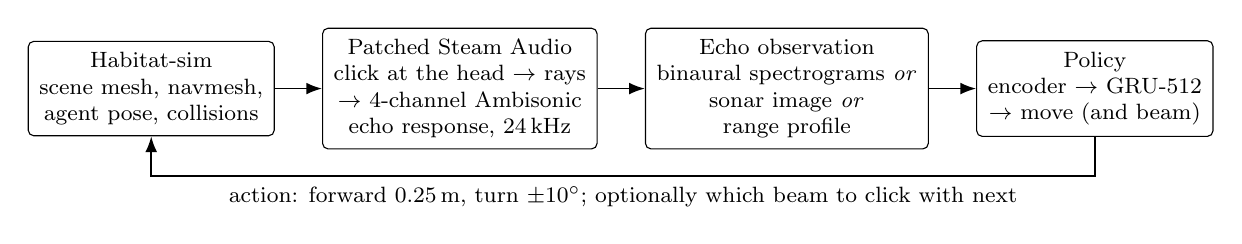
\begin{tikzpicture}[font=\footnotesize, node distance=5mm and 6mm, box/.style={draw, rounded corners=2pt, align=center, inner sep=4pt, minimum height=11mm}, arr/.style={-{Latex[length=2mm]}, semithick}]
\node[box] (hab) {Habitat-sim\\scene mesh, navmesh,\\agent pose, collisions};
\node[box, right=of hab] (sa) {Patched Steam Audio\\click at the head $\rightarrow$ rays\\$\rightarrow$ 4-channel Ambisonic\\echo response, 24\,kHz};
\node[box, right=of sa] (obs) {Echo observation\\binaural spectrograms \emph{or}\\sonar image \emph{or}\\range profile};
\node[box, right=of obs] (pol) {Policy\\encoder $\rightarrow$ GRU-512\\$\rightarrow$ move (and beam)};
\draw[arr] (hab) -- (sa); \draw[arr] (sa) -- (obs); \draw[arr] (obs) -- (pol);
\draw[arr] (pol.south) -- ++(0,-5mm) -| node[pos=0.25, below]{action: forward 0.25\,m, turn $\pm10^\circ$; optionally which beam to click with next} (hab.south);
\end{tikzpicture}
\caption{One environment step. Habitat-sim moves the agent; Steam Audio traces the agent's click on the same triangle mesh; the echo response is converted to one of three observations; a recurrent policy chooses the next movement and, in some configurations, the beam of the next click.}
\label{fig:pipeline}
\end{figure}

\subsection{Embodiment and acoustics}
The agent is a cylinder of radius 0.1\,m with its ears and mouth at 1.5\,m height. Actions follow SoundSpaces: \emph{stop}, \emph{move forward} 0.25\,m, \emph{turn left} $10^\circ$, \emph{turn right} $10^\circ$. Unlike SoundSpaces we disable Habitat's wall sliding: a forward move that would enter an obstacle leaves the agent where it is and is reported as a collision. The agent receives no image at any time.

At every step a click is emitted at the head position and the patched engine traces its reflections on the scene's full triangle mesh (for Replica, the \texttt{mesh\_semantic.ply} files, rotated into Habitat's coordinate frame). Settings: 2{,}048 rays, 4 bounces, 0.3\,s response, first-order Ambisonics (4 channels), 24\,kHz, one Steam Audio thread per environment, air absorption on. \J{8}Every surface has the same material: absorption $(0.10, 0.20, 0.30)$ in the three bands and scattering 0.05. Because source and listener coincide, time zero is the instant of emission and a surface at distance $d$ returns at $2d/c$. The click's own direct sound is not part of the observation.

\subsection{Three echo observations}
\label{sec:obs}

\paragraph{Binaural head scan.} The click is emitted three times, with the head (and a click directivity $((1+\cos\gamma)/2)^2$ around the facing direction, $\gamma$ being the angle from it) turned $-45^\circ$, $0^\circ$ and $+45^\circ$ relative to the body. Each Ambisonic response is decoded to two ears with Steam Audio's default head-related transfer function, resampled to 16\,kHz, and converted to a log-magnitude spectrogram of its first 128\,ms (FFT length 128, hop 16 samples, then averaged over pairs of frames), giving 65 frequency bins $\times$ 64 time frames of 2\,ms $\times$ 2 ears per orientation, 6 channels in total. This is the observation closest to what a human echolocator hears.

\paragraph{Sonar image.} One omnidirectional click per step. In the sparse reconstruction each sample $t$ of the response is one arrival. Its omnidirectional channel $W(t)$ gives the amplitude and its three first-order channels, rearranged to world axes, equal $\sqrt3\,W(t)\,\mathbf u(t)$, where $\mathbf u(t)$ is the unit vector pointing towards the direction of arrival. With the agent's forward, right and up unit vectors $\mathbf f,\mathbf r,\mathbf v$,
\begin{equation}
\varphi(t) = \operatorname{atan2}\!\big(-\mathbf u\!\cdot\!\mathbf r,\ \mathbf u\!\cdot\!\mathbf f\big), \qquad \sin\varepsilon(t) = \mathbf u\!\cdot\!\mathbf v ,
\end{equation}
are the azimuth (positive to the left) and elevation of the arrival in the body frame. We keep the first 128\,ms (3{,}072 samples) and accumulate arrivals into a grid of 64 range bins (48 samples each, i.e.\ 2\,ms of delay or 17\,cm of range, up to 10.9\,m) by 32 azimuth bins ($11.25^\circ$ each, covering the full circle, with ``ahead'' in the centre column):
\begin{equation}
I_0[i,j] = \log\!\Big(1 + 10 \!\!\sum_{t \in \text{bin}(i,j)}\!\! |W(t)|\cos\varepsilon(t)\Big), \qquad
I_1[i,j] = \operatorname{sgn}(S)\log(1 + 10\,|S|),\ \ S = \!\!\sum_{t \in \text{bin}(i,j)}\!\! |W(t)|\sin\varepsilon(t).
\end{equation}
Channel $I_0$ is a top-down polar map of horizontal returns; channel $I_1$ collects returns from the floor (negative) and ceiling (positive) so that they do not clutter $I_0$. The observation has shape $64\times32\times2$. Figure~\ref{fig:sonar}b shows $I_0$ in a shoebox room: the four walls appear at their true distances (errors 3--11\,cm, at most one range bin) and in the correct azimuth columns. No head-related transfer function is involved, which is why this observation needs one traced click instead of three and no binaural decoding.

\paragraph{Range profile and click beams.} To study aiming we remove direction from the echo altogether: the range profile is $P[i]=\log(1+10\sum_{t\in\text{bin}(i)}|W(t)|)$ over the same 64 range bins, a vector of 64 numbers, as a single-microphone ultrasonic range finder would deliver. Direction can then enter only through the click's emission pattern. Steam Audio's source directivity is $|(1-w)+w\cos\gamma|^{p}$ for dipole weight $w$ and power $p$. We use $w=0.5$, $p=8$, i.e.\ $((1+\cos\gamma)/2)^8$, a forward lobe that falls to half its peak value $33^\circ$ off axis, to 0.4\% at $90^\circ$ and to zero directly backwards, aimed at one of five yaw angles relative to the body: $90^\circ$ left, $45^\circ$ left, ahead, $45^\circ$ right, $90^\circ$ right. Figure~\ref{fig:sonar}c confirms that the strongest return of each aimed beam is the wall it points at. (In Experiment~1 the ``learned beam'' agent used an earlier beam set with $w=1$, $p=4$; because of the absolute value this is a figure-of-eight, $|\cos\gamma|^4$, that fires equally backwards. We report those results as run and note this where relevant.)

\begin{figure}[t]
\centering
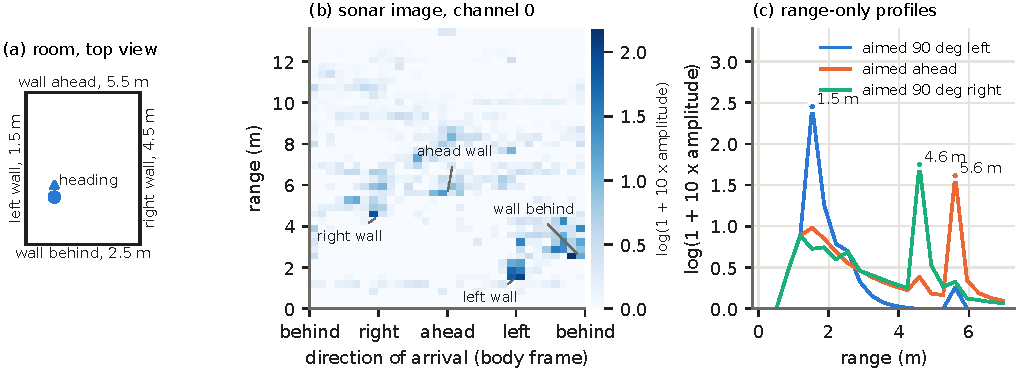
\includegraphics[width=\linewidth]{sonar_shoebox.pdf}
\caption{The echo observations in a 6$\times$8$\times$3\,m shoebox room with the simulation settings of the learning experiments. (a) Agent position and heading. (b) Sonar image channel $I_0$ for one omnidirectional click (4 bounces); the nearest point of each wall appears at its distance and bearing, later entries are multi-bounce paths. (c) Range profiles for a forward-lobe click aimed left, ahead and right (1 bounce): the peak moves to 1.5, 5.6 and 4.6\,m, the distances of the left, front and right walls (1.5, 5.5 and 4.5\,m).}
\label{fig:sonar}
\end{figure}

\subsection{Tasks and rewards}
\paragraph{Exploration in the dark (main experiments).} An episode lasts exactly 300 steps and starts at a random navigable position with a random heading. The floor is divided into square cells of \cell{}; the agent receives $+1$ the first time it enters a cell, $-0.01$ every step, and $-\lambda$ for every step on which it collides ($\lambda=0.05$ in Experiments 1 and 2). \emph{Stop} is treated as \emph{move forward}. The two reported quantities are \textbf{coverage}, the number of distinct cells entered in an episode (the start cell counts, so the minimum is 1), and \textbf{collisions per episode}. In 300 steps an agent can travel at most 75\,m.
\paragraph{Point-goal in the dark (preliminary experiments).} The agent is given the straight-line distance and bearing to a goal at every step and must issue \emph{stop} within 1\,m of it; episodes are limited to 200 steps and start 1--8\,m (geodesic) from the goal. Reward is the decrease in geodesic distance, $-0.01$ per step, $+10$ for success and $-\lambda$ per collision. Metrics are success rate and SPL \citep{anderson2018evaluation}.
\paragraph{Bump sensor.} In exploration every agent, including the blind one, observes one bit: whether its previous action collided.

\subsection{Agents and training}
Each image-like observation is encoded by a three-layer convolutional network (32, 64, 32 channels; kernels $8\times4$, $4\times3$, $3\times3$; strides $(4,2)$, $(2,2)$, 1) followed by a linear layer to 512 units; the range profile by a two-layer perceptron (256, 256); the bump bit by a 16-unit layer. These features are concatenated with a 32-dimensional embedding of the previous action and fed to a GRU \citep{cho2014learning} with 512 units, followed by linear policy and value heads. Agents with a learned beam have a second policy head over beams (sampled independently of the movement) and receive a 16-dimensional embedding of the beam used for the current observation. Parameter counts: 2.09\,M (sonar), 2.12\,M (sonar with beam head), 2.62\,M (head scan), 1.41\,M (range), 0.93\,M (blind).

Training uses PPO \citep{schulman2017proximal} with generalised advantage estimation \citep{schulman2016high}: 14 parallel environments, one per training building; rollouts of 128 steps; 4 epochs over 4 minibatches of whole environment sequences; Adam with learning rate $2.5\times10^{-4}$; $\gamma=0.99$, $\lambda_\text{GAE}=0.95$, clipping 0.2, entropy coefficient 0.02, value coefficient 0.5, gradient-norm clipping 0.5; 1{,}117 updates, i.e.\ 2{,}001{,}664 environment steps.

\paragraph{Auxiliary loss.} All echo agents additionally predict, from the GRU state, $\log(1+d_k)$ for the distance $d_k$ (capped at 10\,m) to the nearest surface along five horizontal directions ($-90^\circ,-45^\circ,0^\circ,45^\circ,90^\circ$ from the heading), with a mean-squared-error loss weighted 0.5. The distances come from ray casts during training and are never observed. The blind agents in Experiment~1 were trained without this loss.
\paragraph{Blank-echo augmentation.} In Experiments 1 and 2 the echo observation of each training step is replaced by zeros with probability 0.05, so that a missing echo is not out of distribution.

\subsection{Buildings and evaluation protocol}
We use the 18 scenes of Replica \citep{straub2019replica}. Four are held out and never seen during training: \texttt{office\_2}, \texttt{frl\_apartment\_4}, \texttt{hotel\_0}, \texttt{room\_2} (navigable area 12.5, 39.6, 16.0 and 13.2\,m$^2$). The other 14 are used for training (5.4--89.0\,m$^2$; Appendix~\ref{app:scenes}).

Every trained agent is evaluated on 30 episodes in each held-out building. The 30 start poses of a building are identical for all agents. Unless stated otherwise we report the \textbf{greedy} policy (most probable action); Appendix~\ref{app:perbuilding} also gives results for sampled actions. For each seed we average over the 120 episodes; we then report the mean and the population standard deviation over the three seeds, written \pmsd{mean}{s.d.} With three seeds these standard deviations are rough, so we also state per-seed values where a conclusion depends on them.

\paragraph{Baselines.} \emph{Bump-and-turn}: move forward until a collision, then turn left by 30--90$^\circ$ (uniformly chosen multiple of $10^\circ$). \emph{Random}: uniformly random actions.
\paragraph{Echo ablations.} On \texttt{office\_2} and \texttt{hotel\_0} each echo agent is re-evaluated with its echo observation replaced (a) by zeros and (b) by an echo observation recorded at a random other pose in the same building (``shuffled''). If an agent's behaviour does not change under (b), it is not using the content of its echoes.

% ======================================================================================================
\section{Preliminary experiments that shaped the design (single seed)}
\label{sec:prelim}
The runs in this section were made with one seed per configuration while the system was being developed. They motivated the main experiments but, as Section~\ref{sec:exp1} shows, single runs differ by several cells and by a factor of two to three in collisions, so they should be read as observations, not as established effects.

\paragraph{P1. Sanity check: reaching a sounding goal.} With SoundSpaces' task definition (a telephone rings at the goal, wall sliding on) in one Habitat test apartment, a PPO agent trained for 1 million steps on binaural spectrograms from our simulator reached the goal in 75\% (greedy) and 79\% (sampled) of 100 unseen start--goal pairs, with SPL 0.67; a random agent reached 2\%. The simulated binaural cues are therefore learnable in the usual way.

\paragraph{P2. Echoes are ignored unless collisions cost something.} For point-goal in the dark in the same apartment, an agent trained with $\lambda=0$ behaved identically with real, shuffled or zeroed echoes. With $\lambda=0.1$, zeroing the echoes at test time multiplied collisions by 3 to 22 while leaving success unchanged, in two seeds of two echo agents (Appendix~\ref{app:prelim}). All later runs use a collision penalty.

\paragraph{P3. Three training buildings do not transfer.} Head-scan agents trained on three buildings for 2 million steps beat blind agents in those buildings (greedy point-goal success 0.88 against 0.73 in the largest) but fell to the blind level in an unseen Matterport3D house (0.18 against 0.21), and shuffling their echoes there changed nothing. This motivated the move to 14 training buildings.

\paragraph{P4. With a goal vector, echoes do not improve success in held-out buildings.} Table~\ref{tab:pointgoal} compares a head-scan echo agent (with auxiliary loss) and a blind agent, both trained for 2 million steps on the 14 Replica training buildings with $\lambda=0.1$. Mean held-out success is 0.38 with echoes and 0.39 without; the blind agent has higher SPL and fewer collisions. Zeroing the echo agent's echoes on \texttt{office\_2} and \texttt{hotel\_0} did not lower its success (0.44 and 0.38) but raised its collisions from 6.1 and 5.2 to 9.6 and 11.0 per episode. The echo agent thus used its echoes only to avoid walls, something the blind agent achieved equally well from the bump bit and the goal vector. We therefore turned to a task without a goal vector.

\begin{table}[t]
\caption{Preliminary result P4 (one seed per agent): point-goal navigation in the dark on the four held-out Replica buildings, greedy policy, 100 episodes per building. Entries are success rate / SPL / collisions per episode. Random actions succeed in 0.01--0.12 of episodes.}
\label{tab:pointgoal}
\centering\small
\begin{tabular}{lcc}
\toprule
Held-out building & Head-scan echo + auxiliary loss & Blind \\
\midrule
office\_2 & 0.34 / 0.31 / 6.1 & 0.39 / 0.38 / 3.8 \\
frl\_apartment\_4 & 0.43 / 0.38 / 6.9 & 0.28 / 0.28 / 3.0 \\
hotel\_0 & 0.37 / 0.30 / 5.2 & 0.45 / 0.44 / 3.0 \\
room\_2 & 0.39 / 0.35 / 4.2 & 0.44 / 0.43 / 4.0 \\
\midrule
Mean & 0.38 / 0.34 / 5.6 & 0.39 / 0.38 / 3.5 \\
\bottomrule
\end{tabular}
\end{table}

\paragraph{P5. \J{9}The collision penalty sets a coverage--collision trade-off.} For exploration with the sonar image and a fixed click, $\lambda=0.02$ gave 41.9 cells and 38.6 collisions per episode on the held-out buildings (one seed); $\lambda=0.05$ gave \pmsd{37.0}{1.5} cells and \pmsd{17.5}{6.7} collisions (three seeds, Experiment~1). With $\lambda=0.1$ a head-scan explorer became progressively more hesitant during training: its checkpoint at 0.5 million steps covered 26.5 and 21.3 cells on \texttt{office\_2} and \texttt{hotel\_0}, its final policy 12.4 and 17.1. We fixed $\lambda=0.05$ for the main experiments.

% ======================================================================================================
\section{Experiment 1: which echo representation helps exploration?}
\label{sec:exp1}

\paragraph{Setup.} Four agents, three seeds each, exploration in the dark with $\lambda=0.05$: (1) \emph{sonar image, fixed click}: one omnidirectional click per step; (2) \emph{sonar image + learned beam}: the agent chooses each step among no click, an omnidirectional click, and a $|\cos\gamma|^4$ beam centred $45^\circ$ left, ahead or $45^\circ$ right, and pays 0.01 reward per click; (3) \emph{head-scan binaural}; (4) \emph{blind}: bump bit only.

\begin{table}[t]
\caption{Experiment 1. Exploration in four held-out Replica buildings (300 steps, greedy policy, 30 episodes per building; mean $\pm$ s.d.\ over 3 seeds). Coverage is the number of distinct \cell{} cells entered. ``Sim.\ speed'' is training throughput with 14 environments on one 8-core CPU and ``Train time'' the wall-clock time for 2 million steps.}
\label{tab:exp1}
\centering\small
\resizebox{\linewidth}{!}{%
\begin{tabular}{lccccc}
\toprule
Agent & Coverage (cells) & Collisions / episode & Path (m) & Sim.\ speed (steps/s) & Train time (h) \\
\midrule
Sonar image, fixed click & \textbf{\pmsd{37.0}{1.5}} & \pmsd{17.5}{6.7} & 31.0 & 490 & 1.13 \\
Sonar image + learned beam & \pmsd{33.6}{4.7} & \textbf{\pmsd{13.2}{2.4}} & 25.8 & 495 & 1.12 \\
Head-scan binaural & \pmsd{26.6}{3.3} & \pmsd{17.4}{3.6} & 18.0 & 181 & 3.08 \\
Blind (bump sensor) & \pmsd{24.5}{3.9} & \pmsd{20.6}{5.3} & 20.5 & 1016 & 0.55 \\
\midrule
Scripted bump-and-turn & 28.0 & 31.8 & 22.2 & -- & -- \\
Random actions & 7.7 & 139.0 & 3.1 & -- & -- \\
\bottomrule
\end{tabular}}
\end{table}

\begin{figure}[t]
\centering
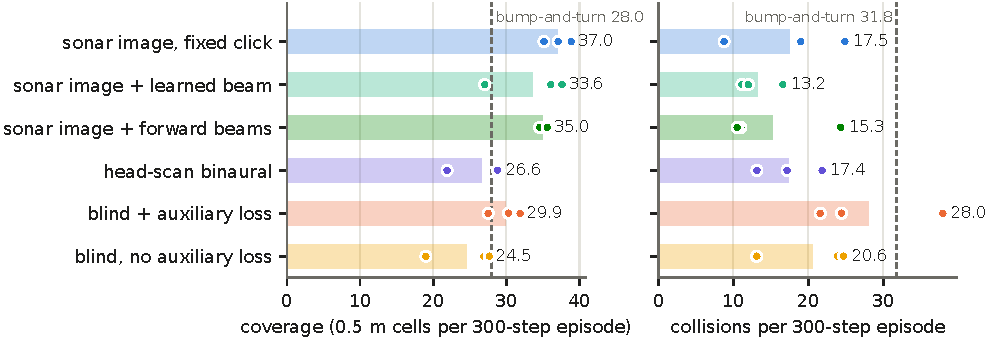
\includegraphics[width=0.95\linewidth]{exp1_sensors.pdf}
\caption{Experiment 1, per-seed results behind Table~\ref{tab:exp1}. Each dot is one training seed (mean over 120 held-out episodes); bars and numbers are means over seeds; the dashed line is the scripted bump-and-turn explorer.}
\label{fig:exp1}
\end{figure}

\paragraph{Result 1: the sonar image clearly improves exploration over blindness.} The sonar agent with a fixed click covers \pmsd{37.0}{1.5} cells against \pmsd{24.5}{3.9} for the blind agent, an increase of 12.5 cells (51\%). The three sonar seeds (38.9, 35.2, 37.1) all exceed the three blind seeds (19.0, 27.0, 27.7). It also exceeds the scripted explorer (28.0) in every held-out building (Appendix~\ref{app:perbuilding}) while colliding about half as often (17.5 against 31.8). In terms of floor area, the sonar agent visits on average 51\%, 35\%, 42\% and 76\% of the navigable area of \texttt{office\_2}, \texttt{frl\_apartment\_4}, \texttt{hotel\_0} and \texttt{room\_2} within 300 steps (25.6, 55.8, 26.9 and 39.9 cells of 0.25\,m$^2$).

\paragraph{Result 2: the binaural head scan is not better than blindness.} The head-scan agent covers \pmsd{26.6}{3.3} cells, within one standard deviation of the blind agent, although each of its steps traces three clicks and decodes three binaural responses, which makes its training 2.7 times slower than the sonar agent's. \J{10}The underlying echo responses are the same in both cases; what differs is that the sonar image hands the policy range and bearing explicitly, whereas the spectrogram leaves the policy to recover them from interaural differences after a head-related transfer function.

\paragraph{Result 3: beam choice in the sonar agent is within seed noise.} The learned-beam variant covers \pmsd{33.6}{4.7} cells with \pmsd{13.2}{2.4} collisions; both differences from the fixed click are smaller than the spread across seeds. The three seeds adopt different habits: clicking on 63\%, 100\% and 85\% of steps and preferring different beams. \J{11}This is unsurprising, because the sonar image already resolves direction, so the beam only re-weights it; and, as noted in Section~\ref{sec:obs}, this beam set also fired backwards. Experiment~2 tests aiming in a setting where it matters.

\paragraph{Do the agents use the content of their echoes?} Table~\ref{tab:ablation} shows the ablations. Both sonar agents lose coverage and gain collisions when echoes are shuffled (fixed click: 26.2 $\to$ 19.8 cells and 21.1 $\to$ 31.8 collisions), so they read geometry from the image. \J{12}With zeroed echoes the fixed-click sonar agent slows down sharply (11.1 cells, 8.7 collisions): despite the 5\% blank-echo augmentation it does not move confidently without echoes. The head-scan agent is essentially unaffected by either ablation (17.4 cells with real echoes, 17.6 shuffled, 18.5 zeroed), which is consistent with Result~2: on these buildings it does not rely on its echoes.

\begin{table}[t]
\caption{Echo ablations on \texttt{office\_2} and \texttt{hotel\_0} (greedy, mean $\pm$ s.d.\ over 3 seeds). Entries are coverage in cells / collisions per episode. ``Shuffled'' replaces each echo observation by one recorded at a random other pose of the same building.}
\label{tab:ablation}
\centering\small
\begin{tabular}{lccc}
\toprule
Agent & Real echoes & Shuffled echoes & Zeroed echoes \\
\midrule
Sonar image, fixed click & \pmsd{26.2}{0.5} / \pmsd{21.1}{8.8} & \pmsd{19.8}{1.2} / \pmsd{31.8}{8.2} & \pmsd{11.1}{4.3} / \pmsd{8.7}{2.7} \\
Sonar image + learned beam & \pmsd{23.4}{3.1} / \pmsd{15.3}{4.3} & \pmsd{14.9}{4.3} / \pmsd{26.0}{12.3} & \pmsd{15.0}{9.4} / \pmsd{19.3}{17.4} \\
Head-scan binaural & \pmsd{17.4}{2.7} / \pmsd{19.3}{6.9} & \pmsd{17.6}{1.4} / \pmsd{21.5}{3.4} & \pmsd{18.5}{2.8} / \pmsd{18.3}{6.6} \\
\addlinespace
Range + learned beam & \pmsd{22.1}{1.0} / \pmsd{16.7}{3.5} & \pmsd{19.9}{5.6} / \pmsd{25.2}{9.9} & \pmsd{15.6}{3.0} / \pmsd{13.1}{3.9} \\
Range + scripted sweep & \pmsd{24.6}{0.5} / \pmsd{25.6}{3.1} & \pmsd{22.7}{0.3} / \pmsd{34.1}{4.2} & \pmsd{16.6}{6.7} / \pmsd{31.3}{27.6} \\
Range + fixed ahead beam & \pmsd{21.6}{3.8} / \pmsd{28.4}{8.1} & \pmsd{20.4}{1.8} / \pmsd{29.8}{9.3} & \pmsd{18.9}{9.6} / \pmsd{25.2}{17.5} \\
Range + omni click & \pmsd{21.5}{5.6} / \pmsd{30.9}{16.3} & \pmsd{20.5}{5.1} / \pmsd{33.9}{17.3} & \pmsd{20.8}{1.2} / \pmsd{65.3}{7.7} \\
\bottomrule
\end{tabular}
\end{table}

\paragraph{Learning curves.} Figure~\ref{fig:curves} shows training coverage and collisions. The blind agents plateau near 33 cells after 0.5 million steps; the sonar agents keep improving to 47 cells at 2 million steps and had not converged. Training coverage is higher than held-out coverage for all agents because the training set contains larger buildings.

\begin{figure}[t]
\centering
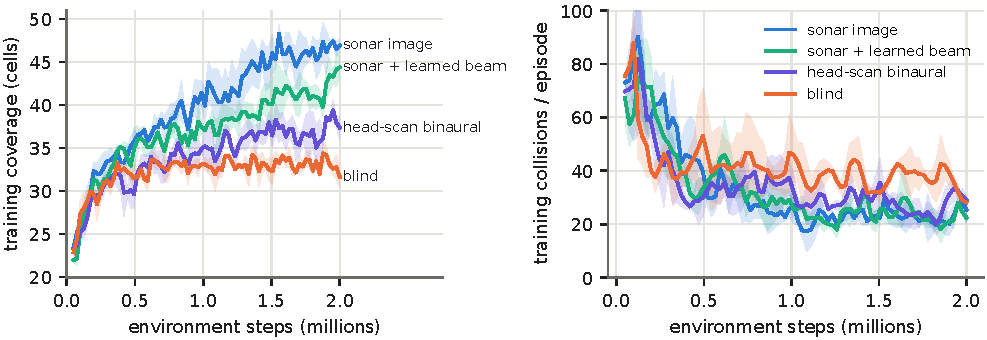
\includegraphics[width=0.95\linewidth]{learning_curves.pdf}
\caption{Experiment 1, training curves on the 14 training buildings (mean over 3 seeds; shading is $\pm1$ s.d.). Left: coverage over the last 100 training episodes. Right: collisions per episode.}
\label{fig:curves}
\end{figure}

% ======================================================================================================
\section{Experiment 2: does learned click aiming help when the beam is the only source of direction?}
\label{sec:exp2}

\paragraph{Setup.} All four agents observe the 64-number range profile and the bump bit and are trained exactly as in Experiment~1 (including the auxiliary loss and blank-echo augmentation). They differ only in how the click is emitted: (1) \emph{learned beam}: each step the agent chooses one of the five forward beams of Section~\ref{sec:obs} or no click, at a cost of 0.01 per click; (2) \emph{scripted sweep}: the beam cycles through the five directions, one per step, in fixed order (the agent is not told the current direction and must track the cycle in memory); (3) \emph{fixed ahead beam}; (4) \emph{omnidirectional click}.

\begin{table}[t]
\caption{Experiment 2. Range-only echo observation with four ways of emitting the click; same protocol as Table~\ref{tab:exp1} (mean $\pm$ s.d.\ over 3 seeds). The first and last rows repeat Experiment~1 for reference.}
\label{tab:exp2}
\centering\small
\resizebox{\linewidth}{!}{%
\begin{tabular}{lcccc}
\toprule
Agent & Coverage (cells) & Collisions / episode & Path (m) & Clicks per step (seeds 1, 2, 3) \\
\midrule
Sonar image, fixed click (Exp.~1) & \pmsd{37.0}{1.5} & \pmsd{17.5}{6.7} & 31.0 & 1 \\
\addlinespace
Range + fixed ahead beam & \pmsd{32.0}{3.2} & \pmsd{29.3}{11.5} & 24.4 & 1 \\
Range + scripted sweep & \pmsd{30.4}{0.3} & \pmsd{24.4}{3.3} & 23.5 & 1 \\
Range + omni click & \pmsd{28.5}{8.1} & \pmsd{29.3}{14.4} & 20.3 & 1 \\
Range + learned beam & \pmsd{27.7}{1.4} & \textbf{\pmsd{15.4}{2.0}} & 17.9 & 0.38, 0.96, 0.76 \\
\addlinespace
Blind (Exp.~1) & \pmsd{24.5}{3.9} & \pmsd{20.6}{5.3} & 20.5 & 0 \\
\bottomrule
\end{tabular}}
\end{table}

\begin{figure}[t]
\centering
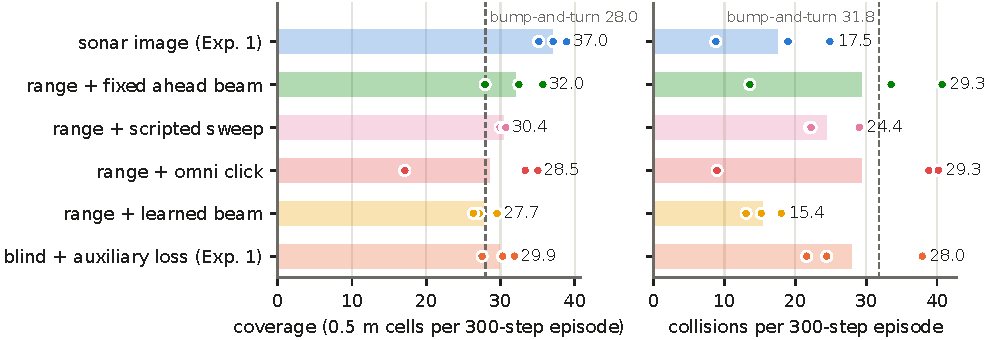
\includegraphics[width=0.95\linewidth]{exp2_range.pdf}
\caption{Experiment 2, per-seed results behind Table~\ref{tab:exp2}. Dots are seeds; bars and numbers are means; the dashed line is the scripted bump-and-turn explorer.}
\label{fig:exp2}
\end{figure}

\paragraph{Result 4: direction in the echo is worth 5 to 9 cells.} Every range-only agent lies between the blind agent (24.5 cells) and the sonar-image agent (37.0 cells). The best range-only mean, 32.0 cells, is 5.0 below the sonar image; the learned-beam agent is 9.3 below.

\paragraph{Result 5: learned aiming does not increase coverage, but produces the safest explorer.} The learned-beam agent covers \pmsd{27.7}{1.4} cells, fewer than the fixed ahead beam (\pmsd{32.0}{3.2}) and the scripted sweep (\pmsd{30.4}{0.3}). Its collisions are the lowest of any agent in this paper with the smallest spread, \pmsd{15.4}{2.0} per episode (seeds: 13.0, 18.0, 15.2), and its path is the shortest (17.9\,m): \J{13}it trades distance travelled for not hitting things. By contrast the fixed-beam and omnidirectional agents vary between 9 and 41 collisions per episode across seeds (13.6, 33.6, 40.8 and 38.8, 40.2, 9.0).

\paragraph{Result 6: agents ration clicks to different degrees.} With a click cost equal to the per-step time cost (0.01), seed 1 of the learned-beam agent stays silent on 62\% of steps (clicks on 21--46\% of steps depending on the building), seed 3 on 24\%, and seed 2 clicks on 96\% of steps. Preferred beams differ by seed: seed 1 clicks mostly $45^\circ$ left (14--20\% of steps, depending on the building) and $90^\circ$ right (3--17\%), seed 2 mostly ahead (33--54\%), seed 3 mostly $45^\circ$ left (22--46\%). Zeroing the range profile reduces the learned-beam agents' coverage from 22.1 to 15.6 cells on the two ablation buildings (Table~\ref{tab:ablation}), so the echoes obtained with the chosen beams are used.

\paragraph{Result 7: a scripted sweep is the most reproducible range-only sensor.} Its three seeds cover 30.0, 30.6 and 30.7 cells. Sweeping gives the recurrent policy five directions every five steps without any learning of where to look.

% ======================================================================================================
\section{Experiment 3: what do the agents remember?}
\label{sec:probe}

\paragraph{Setup.} We take the 12 trained agents of Experiment~1 and roll each out with sampled actions, without further training, for 3{,}000 steps in each of the 14 training buildings and 6{,}000 steps in each of the 4 held-out buildings. At every step we store the 512-dimensional GRU state $h_t$, a reduced copy $x_t$ of the current observation (the echo observation average-pooled to at most 512 numbers, plus the bump bit; for the blind agent $x_t$ is the bump bit alone), and two binary labels for each cell of an $11\times11$ grid of \cell{} cells centred on the agent and aligned with its heading (5.5\,m $\times$ 5.5\,m): \emph{walkable}, whether the cell centre lies on the navigation mesh, and \emph{visited}, whether the agent has entered that cell earlier in the episode. This yields 41{,}860 training and 23{,}920 held-out samples per agent. On average 29\% of cells are walkable and 11\% visited.

For each agent and each label we train a decoder (one hidden layer of 256 units, sigmoid outputs for the 120 non-centre cells; Adam, learning rate $10^{-3}$, weight decay $10^{-4}$, 15 epochs, batch size 512, standardised inputs) on the samples from the training buildings and report the area under the ROC curve (AUROC) on the held-out buildings, averaged over cells; 0.5 is chance. We do this once with $h_t$ as input and once with $x_t$. Linear decoders give the same ordering (Appendix~\ref{app:probe}).

Visited cells are always walkable, so a decoder could score above chance on \emph{visited} merely by recognising walls. We therefore evaluate \emph{visited} only over the cells that are walkable in the sample at hand (``path memory''): of the floor that the agent could have stepped on, which part has it actually stepped on? No single echo contains this information.

\begin{figure}[t]
\centering
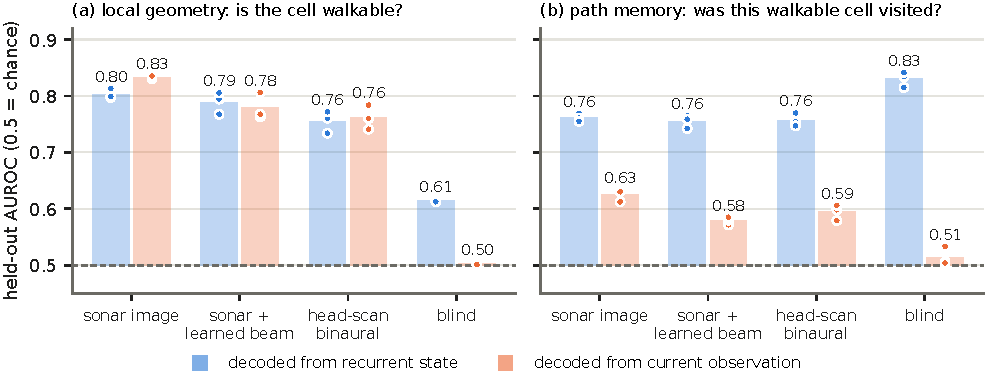
\includegraphics[width=0.95\linewidth]{probe.pdf}
\caption{Experiment 3. Held-out AUROC of decoders that read the agent's recurrent state (blue) or only its current observation (orange). Dots are the three seeds of each agent, bars and numbers their mean. (a) Which of the 120 surrounding cells are walkable. (b) Which walkable cells the agent has already visited in this episode.}
\label{fig:probe}
\end{figure}

\paragraph{Result 8: all agents carry a record of their own path, readable in unseen buildings.} From the recurrent state, path memory is decoded with AUROC \pmsd{0.762}{0.006} (sonar, fixed click), \pmsd{0.755}{0.010} (sonar, learned beam), \pmsd{0.757}{0.009} (head scan) and \pmsd{0.830}{0.011} (blind). From the current observation it is \pmsd{0.625}{0.009}, \pmsd{0.579}{0.005}, \pmsd{0.594}{0.011} and \pmsd{0.515}{0.013}. The agents were trained only with the coverage reward (and, for echo agents, the wall-distance loss); nothing asked them to store where they had been.

\paragraph{Result 9: the blind agents remember their path best.} Their path-memory AUROC of 0.830 exceeds that of every echo agent ($\leq 0.762$) in all three seeds. \J{14}An agent that cannot sense walls can avoid re-covering ground only by integrating its own movements; an agent that hears the room has other cues for where open, unvisited space lies.

\paragraph{Result 10: echo agents perceive local geometry rather than remember it.} For walkable cells, the sonar agent's current observation decodes better than its memory (\pmsd{0.832}{0.002} against \pmsd{0.803}{0.007}); for the learned-beam and head-scan agents the two are equal within noise (0.779 against 0.789; 0.761 against 0.755). \J{15}The recurrent state thus retains somewhat less geometric information than a pooled copy of the latest echo contains. The blind agents' memory holds a weak map of walkable space built from bumps and movement alone (\pmsd{0.614}{0.002}; the bump bit by itself gives 0.503).

% ======================================================================================================
\section{Experiment 4: erasing memory during an episode}
\label{sec:wipe}
Experiment~3 shows what can be read out of memory, not whether the agents need it. Here we remove it.

\paragraph{Setup.} We re-evaluate trained agents on \texttt{office\_2} and \texttt{hotel\_0} (greedy policy, the same 30 start poses per building as before, 3 seeds) while setting the GRU state to zero every $N$ steps. The zero state is the state every training episode starts with, so the erased state itself is familiar to the policy. The embedding of the previous action (and beam) is still supplied. $N=20$ removes everything older than at most 20 steps (at most 5\,m of travel); $N=1$ removes memory entirely, so that the action depends only on the current observation and the previous action. The agents are the blind agent without auxiliary loss, the sonar-image agents with fixed click and with the figure-of-eight learned beam of Experiment~1 and the range + learned-beam agent of Experiment~2.

\begin{table}[t]
\caption{Experiment 4. Exploration on \texttt{office\_2} and \texttt{hotel\_0} with the recurrent memory erased every 20 steps or every step (greedy, mean $\pm$ s.d.\ over 3 seeds). Entries: coverage in cells / collisions per episode / path length in metres.}
\label{tab:wipe}
\centering\small
\resizebox{\linewidth}{!}{%
\begin{tabular}{lccc}
\toprule
Agent & Memory intact & Erased every 20 steps & Erased every step \\
\midrule
Blind & \pmsd{21.3}{3.2} / \pmsd{22.2}{6.1} / 18.9 & \pmsd{18.2}{2.4} / \pmsd{17.6}{2.1} / 14.6 & \pmsd{3.2}{0.0} / \pmsd{1.0}{0.0} / 1.0 \\
Sonar image, fixed click & \pmsd{25.4}{0.8} / \pmsd{22.7}{9.5} / 23.6 & \pmsd{27.5}{1.0} / \pmsd{20.8}{8.6} / 24.6 & \pmsd{20.9}{2.4} / \pmsd{71.4}{6.9} / 14.7 \\
Sonar image + learned beam & \pmsd{23.3}{3.7} / \pmsd{15.1}{4.3} / 20.9 & \pmsd{23.9}{1.8} / \pmsd{17.9}{4.3} / 19.8 & \pmsd{16.3}{2.8} / \pmsd{89.3}{15.5} / 12.6 \\
Range + learned beam & \pmsd{21.8}{1.5} / \pmsd{16.9}{3.2} / 15.1 & \pmsd{24.2}{1.8} / \pmsd{18.1}{2.8} / 15.5 & \pmsd{22.8}{1.8} / \pmsd{78.6}{8.0} / 14.5 \\
\bottomrule
\end{tabular}
}
\end{table}

\paragraph{Result 11: only the blind agents lose coverage when memory older than 20 steps is erased.} Their coverage falls from \pmsd{21.3}{3.2} to \pmsd{18.2}{2.4} cells ($-15\%$), and it falls in every seed ($16.8\to15.6$, $23.2\to17.5$, $23.8\to21.3$). For the three echo agents coverage does not fall in the mean (sonar, fixed click: $25.4\to27.5$; sonar, learned beam: $23.3\to23.9$; range, learned beam: $21.8\to24.2$) and collisions change by less than their standard deviation over seeds. \J{23}Taken with Result~9, this supports the reading that blind explorers rely on a longer record of their own path, whereas agents that hear the room can re-derive what they need from the next echo.

\paragraph{Result 12: without any memory, echo agents still cover ground but collide three to six times more; blind agents stop.} With the state erased at every step the sonar agent with a fixed click still covers \pmsd{20.9}{2.4} cells (82\% of its normal coverage), the sonar agent with a learned beam \pmsd{16.3}{2.8} (70\%), and the range + learned-beam agent \pmsd{22.8}{1.8} (no loss), but their collisions rise from 22.7 to 71.4, from 15.1 to 89.3 and from 16.9 to 78.6 per episode. To see whether these extra collisions are repeats, we logged the position and heading of every collision and counted those that occurred within 5\,cm and $5^\circ$ of an earlier collision in the same episode. With memory intact such repeats make up \pmsd{14}{6}\% of the collisions of the sonar agent with a fixed click, \pmsd{13}{3}\% for the sonar agent with a learned beam and \pmsd{3}{1}\% for the range + learned-beam agent; without memory they make up \pmsd{47}{20}\%, \pmsd{52}{14}\% and \pmsd{18}{7}\% (per-seed values for the first agent: 22\%, 72\%, 48\%). None of these repeats happens on the step directly after the earlier collision; the agent turns away and comes back later. About half of the additional collisions of the memoryless sonar agents are thus returns to an obstacle already hit from the same direction, and the rest are collisions at new places, so short-term memory both prevents such returns and lowers the collision rate elsewhere. The agents' choice of where to go is largely reactive to the current echo. The memoryless blind agent moves 1.0\,m, collides once and makes no further progress (3.2 cells in all three seeds): its only inputs are then one bump bit and its previous action.

\paragraph{Repeatability of the evaluation.} The ``memory intact'' column repeats the evaluation of Table~\ref{tab:ablation} on the same start poses. For the blind agents, which use no acoustics, the two evaluations agree exactly (per-seed coverage 16.8, 23.2, 23.8 in both). For the sonar agent with a fixed click the three-seed mean is 25.4 here against 26.2 there, and for the range + learned-beam agent 21.8 against 22.1: the reason is that Steam Audio draws new random ray directions for every simulation run, whatever the number of threads. Two clicks emitted at the same pose with identical settings give sonar images whose channel $I_0$ correlates at 0.94 and 0.97 on average in two buildings (20 poses each; the strongest cell is the same in all 40 pairs) and range profiles that correlate at 0.999 (Appendix~\ref{app:extra}). The echo observations are thus noisy at a fixed pose, evaluations are not bit-reproducible, and differences of up to about one cell in a three-seed mean should not be interpreted.


% ======================================================================================================
\section{Discussion}

\paragraph{Why echoes helped exploration but not goal reaching.} With a goal vector the agent already knows where to go; what it lacks is knowledge of obstacles on the way, and in small apartments a bump sensor plus the goal vector suffices to route around them at the cost of a few collisions (3.5 per episode for the blind agent in Table~\ref{tab:pointgoal}). In exploration the agent must decide where unvisited open space is, and echoes carry exactly that: the sonar image shows the distance to walls in every direction. \J{16}This suggests that benchmarks intended to measure the value of echolocation should not provide a goal vector.

\paragraph{Representation over raw signal.} The head-scan agent received strictly more acoustic simulation per step than the sonar agent and performed no better than a blind agent, whereas a deterministic transformation of one first-order Ambisonic response into range and bearing made echoes useful within 2 million steps. \J{17}We do not claim that binaural input cannot work, only that at this training budget and with this encoder it did not, while the cheaper explicit representation did. \J{18}For a physical device the sonar image needs a four-capsule (tetrahedral) microphone and a pulse-compressed emitter instead of two ears; its main real-world difficulty, which our simulator does not reproduce, is that arrivals overlapping within one sample blur the intensity-vector direction.

\paragraph{Active sensing.} When aiming was necessary for direction (Experiment~2), agents did learn to aim and, in one seed out of three, to stay silent most of the time, but this bought safety and sensing economy, not coverage. \J{19}A plausible reason is that the coverage reward favours continuous forward motion, for which a fixed forward-looking beam is sufficient, while looking sideways mainly helps to avoid side collisions.

\paragraph{Memory.} The probe results show a division of labour between perception and memory that depends on the sensor: agents that sense walls keep geometry in the observation and a moderate path record in memory; agents that do not sense walls keep a stronger path record. Experiment~4 shows that this difference is functional: only the blind agents lose coverage when the record is truncated to 20 steps, and the echo agents' choice of direction survives even complete removal of memory, at the price of many more collisions.

% ======================================================================================================
\section{Limitations}
\begin{itemize}
\item \textbf{Simulation only, geometric acoustics.} The engine has no diffraction, a single material for all surfaces in our setup, three frequency bands, and the $\cos\theta$ deficit of Section~\ref{sec:deviations}. The sparse reconstruction delivers one arrival per sample, which makes the intensity-vector direction cleaner than in real recordings. No claim about real-world performance follows from these results.
\item \textbf{Three seeds.} Standard deviations over three seeds are imprecise. We make claims only where all seeds of one agent exceed all seeds of another (sonar image against blind coverage; blind against echo-agent path memory) or state explicitly that a difference is within seed noise.
\item \textbf{Small buildings, one dataset.} The held-out buildings have 12.5--39.6\,m$^2$ of navigable floor; three of the four are single rooms. Larger multi-room buildings may change the ranking, in particular for path memory.
\item \textbf{Training budget.} Sonar agents were still improving at 2 million steps (Figure~\ref{fig:curves}); the head-scan agents may need more.
\item \J{20}\textbf{Confounds we did not remove.} The blind agents of Experiment~1 were trained without the auxiliary wall-distance loss that the echo agents had. The learned-beam agent of Experiment~1 used figure-of-eight beams. The comparison between collision penalties in P5 also differs in blank-echo augmentation.
\item \textbf{Probe.} The observation baseline of Experiment~3 is a pooled copy of the observation, not the full observation, and the decoders are small; AUROC values are lower bounds on what is decodable.
\item \textbf{Greedy evaluation.} Sampled-action results (Appendix~\ref{app:perbuilding}) show the same ranking with smaller gaps for coverage and more collisions.
\end{itemize}

\section{Conclusion}
A 172-line patch turns Steam Audio into a simulator in which single echoes arrive at the correct sample, and makes it possible to study learned echolocation in real building geometry at several hundred environment steps per second on one desktop CPU. In that setting, echoes of the agent's own clicks did not help reach a goal whose position was given, but increased the floor area explored in unseen buildings by half when presented as a range-by-bearing image, and not at all when presented as binaural spectrograms. Aiming the click was learnable but made agents careful rather than fast. Probing and memory erasure showed that all explorers remember their own path, that blind explorers depend on that memory most, and that echo-guided explorers need memory mainly to avoid repeating collisions.

\subsubsection*{Reproducibility statement}
The repository accompanying this submission contains the patch against Steam Audio 4.8.1 and build scripts, the C validation harness and its analysis, the Python binding, the environment, training and evaluation code, the shell scripts with the exact command line of every run, the evaluation logs and per-update training logs of every run reported here, and the script that regenerates all figures and the per-building table from those logs. \J{21}Policy checkpoints (about 30\,MB each) and raw impulse responses are not included in the repository because of their size. All experiments ran on one workstation with an AMD Ryzen~7 5800X (8 cores), 94\,GB of memory and one NVIDIA RTX~2080~Ti; the acoustics run on the CPU and the GPU is used for the policy only. The 24 training runs of Experiments 1 and 2 took 30.7 hours in total.

\subsubsection*{Use of AI assistance}
\J{22}The simulator patch, environment, training and analysis code, the experiment scripts and the first draft of this manuscript were written with an AI coding assistant working under the direction of the author, who posed the research questions, selected the experiments and takes responsibility for all content. Every number in the paper was produced by the released scripts from the released logs.

\bibliography{refs}
\bibliographystyle{tmlr}

\appendix
\section{Simulator validation in full}
\label{app:validation}

All single-wall tests use a C program that calls the Steam Audio C API directly: one planar wall (200\,m $\times$ 200\,m unless stated), one source, one listener, one bounce, first-order Ambisonics, 48\,kHz, 65{,}536 rays for the stock library and 262{,}144 rays for the patched library. The impulse response is obtained by sending a unit impulse through the engine's convolution reflection effect after one silent frame. About 100 scenarios are run per library and compared with closed-form predictions by a script that writes a pass/fail list. Table~\ref{tab:val-stock} lists the checks on the unmodified library and Table~\ref{tab:val-patched} those on the patched library.

\begin{table}[h]
\caption{Checks on the unmodified Steam Audio 4.8.1 library (25 of 25 pass).}
\label{tab:val-stock}
\centering\small
\begin{tabular}{p{0.2\linewidth}p{0.75\linewidth}}
\toprule
Quantity & Result \\
\midrule
Reflection delay & reflection energy appears in the correct 10\,ms bin of $(r_\text{refl}-r_\text{direct})/c$ for 13 wall distances and 5 source distances \\
Speed of sound & bin indices at five path lengths chosen to separate the two hypotheses agree with 340\,m/s in 5 of 5 cases and with 343\,m/s in 2 of 5 \\
Absorption & $E(\alpha)/E(0)=1-\alpha$ to four decimals; per-band spectral ratios within 0.02 of the band-filter model \\
Distance & $E \propto r_\text{refl}^{-2}$, log--log slope $-1.998$, spread 0.24\% over 6--103\,m; energy follows the image-source path length, not the source-to-wall distance \\
Absolute level & measured 5.60 against 5.93 predicted from the noise reconstruction constants \\
Direction & first-order channels point to the image source; N3D gain 1.715 (expected 1.732) \\
Scattering & on a 2$\times$2\,m panel $E(s)/E(0)=1+s(R-1)$ with $R=0.453$ (Lambertian/specular ratio), within 0.015 \\
Finite panel & specular point on the panel: 0.998 of the infinite wall; specular point 5\,m off the panel: $4\times10^{-12}$ \\
Direct path & occlusion 0 behind the wall, 1 otherwise; attenuation $1/\max(r,1\,\text{m})$; air absorption $e^{-k_b r}$ exact \\
Geometry & reversed triangle winding gives an identical reflection; a source behind the wall gives none; an empty scene gives a zero response \\
Ray count & 65{,}536 rays within $10^{-4}$ of 262{,}144 rays in energy; 1{,}024 rays within 4\% \\
\bottomrule
\end{tabular}
\end{table}

\begin{table}[h]
\caption{Checks on the patched library with one-sample bins and sparse reconstruction (26 of 26 pass).}
\label{tab:val-patched}
\centering\small
\begin{tabular}{p{0.2\linewidth}p{0.75\linewidth}}
\toprule
Quantity & Result \\
\midrule
Arrival time & onset sample equals $\lfloor (r_\text{refl}-1\,\text{cm}-r_\text{direct})f_s/c\rfloor$ within 1 sample for 13 wall distances from 1 to 15\,m; fitted speed of sound 340.01\,m/s \\
Long range & 34--102\,m paths: onset within 0.8 sample with $10^6$ rays; with 65{,}536 rays only 1--2 rays fall in each sample-wide ring of the specular spot and onsets jitter by a few samples \\
Glossy tail & centroid minus onset is 0.87--0.98 of the predicted mean excess path $2w/(n+1)$ for wall distances $w=1.5$--40\,m \\
Distance & $E\,r^2$ constant to 0.3\% over 3--80\,m (source at listener) and 0.26\% over 6--103\,m (source apart); slopes $-2.003$ and $-1.998$ \\
Absolute level & $E\,/\,[(1+2/n)/(4\pi r^2)]=12.2$ against $4\pi=12.57$ \\
Absorption & $1-\alpha$ to four decimals; band ratios within 0.024 of the complementary-filter model \\
Air absorption & per band within 0.018 of $e^{-k_b d}$ evaluated at each sample's distance \\
Scattering & infinite diffuse wall: energy ratio 2.02 against 1.96 analytic; 2$\times$2\,m panel within 0.016 \\
Direction, occlusion, transmission, two-sidedness, empty scene & same outcome as for the stock library \\
\bottomrule
\end{tabular}
\end{table}

\paragraph{Shoebox room.} 6$\times$4$\times$3\,m, source and listener at different positions, 262{,}144 rays, patched library. (1) All six first-order echoes begin at the sample predicted by the image-source model. (2) Their energies are 0.92--1.15 of the image-source prediction once the $\cos\theta$ factor of Section~\ref{sec:deviations} is applied at the last wall, and 0.70--1.04 of a pure mirror model. (3) Their energy-weighted direction vectors differ from the predicted direction vectors by at most 0.15. (4) The energy decay over the first 40\,ms is within 1.05\,dB of a three-bounce image-source model with the $\cos\theta$ factor. (5) Reverberation time by Schroeder backward integration, divided by the Eyring prediction, is 0.91, 1.04, 1.11 for diffuse walls with $\alpha=0.1,0.3,0.5$ and 1.05, 1.17, 1.24 for specular walls. (6) Steam Audio's own parametric reverberation estimate agrees with the Schroeder value of its impulse response to 1\%. (7) The Embree build gives the same ratios. Seven of seven checks pass.

\paragraph{Echo timing inside the learning environment.} In a Habitat test apartment (382{,}000 triangles), at 12 random poses, the first echo in the binaural click response arrived at $2d/c$ for the nearest surface distance $d$ with a maximum error of 0.7\,ms after removing the 3.25\,ms latency of the binaural decoder.

\section{Buildings}
\label{app:scenes}
Table~\ref{tab:scenes} lists the navigable floor area of every Replica scene as reported by Habitat's navigation mesh for an agent of radius 0.1\,m and height 1.5\,m.

\begin{table}[h]
\caption{Replica scenes and navigable area. One training environment runs in each of the 14 training scenes.}
\label{tab:scenes}
\centering\small
\begin{tabular}{lr@{\hskip 2em}lr@{\hskip 2em}lr}
\toprule
Training scene & m$^2$ & Training scene & m$^2$ & Held-out scene & m$^2$ \\
\midrule
apartment\_0 & 89.0 & frl\_apartment\_5 & 44.2 & office\_2 & 12.5 \\
apartment\_1 & 52.9 & office\_0 & 7.6 & frl\_apartment\_4 & 39.6 \\
apartment\_2 & 44.7 & office\_1 & 5.4 & hotel\_0 & 16.0 \\
frl\_apartment\_0 & 40.4 & office\_3 & 20.3 & room\_2 & 13.2 \\
frl\_apartment\_1 & 42.0 & office\_4 & 22.9 & & \\
frl\_apartment\_2 & 39.2 & room\_0 & 17.1 & & \\
frl\_apartment\_3 & 42.3 & room\_1 & 11.1 & & \\
\bottomrule
\end{tabular}
\end{table}

\section{Per-building and sampled-action results}
\label{app:perbuilding}
Table~\ref{tab:perbuilding} gives the greedy-policy results of every seed in every held-out building for Experiments 1 and 2. Table~\ref{tab:sampled} repeats Tables~\ref{tab:exp1} and~\ref{tab:exp2} for actions sampled from the policy distribution.

\begin{table}[h]
\caption{Greedy-policy results per held-out building and seed (30 episodes each).}
\label{tab:perbuilding}
\centering\footnotesize
\begin{tabular}{llrrrrrrrr}
\toprule
 & & \multicolumn{4}{c}{Coverage (cells)} & \multicolumn{4}{c}{Collisions per episode} \\
\cmidrule(lr){3-6}\cmidrule(lr){7-10}
Agent & Building & seed 1 & seed 2 & seed 3 & mean & seed 1 & seed 2 & seed 3 & mean \\
\midrule
Sonar image, fixed click & office\_2 & 24.4 & 24.5 & 27.9 & 25.6 & 19.0 & 16.8 & 40.1 & 25.3 \\
 & frl\_apartment\_4 & 58.9 & 51.6 & 56.8 & 55.8 & 28.7 & 9.2 & 22.6 & 20.2 \\
 & hotel\_0 & 29.0 & 26.7 & 25.0 & 26.9 & 18.0 & 7.0 & 25.9 & 17.0 \\
 & room\_2 & 43.3 & 37.8 & 38.7 & 39.9 & 10.2 & 2.1 & 10.9 & 7.7 \\
\addlinespace
Sonar image + learned beam & office\_2 & 27.0 & 23.6 & 19.5 & 23.4 & 23.4 & 13.6 & 9.1 & 15.4 \\
 & frl\_apartment\_4 & 52.3 & 63.5 & 47.7 & 54.5 & 14.5 & 11.7 & 9.5 & 11.9 \\
 & hotel\_0 & 27.5 & 23.2 & 19.6 & 23.4 & 19.3 & 10.1 & 16.2 & 15.2 \\
 & room\_2 & 43.7 & 33.9 & 21.3 & 33.0 & 9.1 & 9.2 & 13.3 & 10.5 \\
\addlinespace
Head-scan binaural & office\_2 & 10.5 & 17.8 & 19.2 & 15.8 & 12.2 & 20.2 & 27.8 & 20.1 \\
 & frl\_apartment\_4 & 43.0 & 37.1 & 37.9 & 39.3 & 21.1 & 19.5 & 25.2 & 21.9 \\
 & hotel\_0 & 16.7 & 21.1 & 18.8 & 18.9 & 10.3 & 16.7 & 28.6 & 18.5 \\
 & room\_2 & 17.4 & 40.1 & 39.3 & 32.3 & 9.0 & 12.3 & 5.8 & 9.0 \\
\addlinespace
Blind, no auxiliary loss & office\_2 & 17.8 & 24.8 & 26.3 & 23.0 & 14.0 & 27.5 & 25.4 & 22.3 \\
 & frl\_apartment\_4 & 23.6 & 32.9 & 32.1 & 29.5 & 12.7 & 21.1 & 22.5 & 18.8 \\
 & hotel\_0 & 15.8 & 21.7 & 21.3 & 19.6 & 13.2 & 26.3 & 27.1 & 22.2 \\
 & room\_2 & 18.8 & 28.4 & 31.0 & 26.1 & 12.6 & 20.7 & 23.8 & 19.0 \\
\addlinespace
Blind + auxiliary loss & office\_2 & 29.6 & 25.4 & 23.6 & 26.2 & 25.8 & 23.0 & 46.2 & 31.7 \\
 & frl\_apartment\_4 & 34.1 & 31.2 & 37.6 & 34.3 & 21.6 & 19.1 & 33.0 & 24.6 \\
 & hotel\_0 & 21.8 & 22.7 & 24.0 & 22.8 & 29.6 & 24.9 & 40.8 & 31.8 \\
 & room\_2 & 35.7 & 30.8 & 42.4 & 36.3 & 20.7 & 19.4 & 31.7 & 23.9 \\
\addlinespace
Sonar + learned forward beams & office\_2 & 25.9 & 16.2 & 28.8 & 23.6 & 17.0 & 14.5 & 44.0 & 25.2 \\
 & frl\_apartment\_4 & 58.6 & 58.4 & 59.7 & 58.9 & 5.9 & 11.3 & 11.6 & 9.6 \\
 & hotel\_0 & 23.9 & 23.6 & 30.4 & 26.0 & 11.7 & 11.1 & 21.9 & 14.9 \\
 & room\_2 & 30.5 & 40.0 & 23.6 & 31.4 & 9.4 & 5.2 & 19.7 & 11.4 \\
\addlinespace
Range + learned beam & office\_2 & 23.5 & 26.4 & 25.3 & 25.1 & 15.3 & 21.5 & 18.9 & 18.6 \\
 & frl\_apartment\_4 & 34.8 & 36.8 & 28.5 & 33.4 & 16.5 & 14.9 & 14.5 & 15.3 \\
 & hotel\_0 & 18.5 & 20.3 & 18.7 & 19.2 & 9.7 & 20.5 & 14.3 & 14.8 \\
 & room\_2 & 31.7 & 34.7 & 32.9 & 33.1 & 10.7 & 15.2 & 13.1 & 13.0 \\
\addlinespace
Range + scripted sweep & office\_2 & 24.9 & 26.2 & 27.5 & 26.2 & 21.3 & 30.7 & 36.4 & 29.5 \\
 & frl\_apartment\_4 & 35.5 & 34.2 & 37.5 & 35.7 & 27.2 & 21.3 & 34.7 & 27.7 \\
 & hotel\_0 & 23.7 & 22.2 & 23.1 & 23.0 & 23.0 & 19.1 & 22.9 & 21.7 \\
 & room\_2 & 35.7 & 39.7 & 34.7 & 36.7 & 16.6 & 17.8 & 22.2 & 18.9 \\
\addlinespace
Range + fixed ahead beam & office\_2 & 22.5 & 29.2 & 18.9 & 23.5 & 22.5 & 40.5 & 49.3 & 37.4 \\
 & frl\_apartment\_4 & 42.4 & 43.7 & 41.5 & 42.5 & 12.0 & 46.8 & 76.2 & 45.0 \\
 & hotel\_0 & 20.5 & 23.4 & 15.1 & 19.7 & 11.9 & 30.9 & 15.5 & 19.4 \\
 & room\_2 & 44.5 & 46.5 & 36.2 & 42.4 & 7.9 & 16.0 & 22.0 & 15.3 \\
\addlinespace
Range + omni click & office\_2 & 26.4 & 25.0 & 11.8 & 21.1 & 39.3 & 43.2 & 5.1 & 29.2 \\
 & frl\_apartment\_4 & 34.8 & 41.8 & 30.8 & 35.8 & 45.6 & 43.6 & 16.8 & 35.3 \\
 & hotel\_0 & 24.0 & 26.3 & 15.5 & 21.9 & 44.1 & 43.2 & 10.6 & 32.6 \\
 & room\_2 & 48.2 & 47.0 & 10.3 & 35.2 & 26.4 & 30.8 & 3.3 & 20.2 \\
\bottomrule
\end{tabular}

\end{table}

\begin{table}[h]
\caption{Results with sampled actions on the four held-out buildings (mean $\pm$ s.d.\ over 3 seeds).}
\label{tab:sampled}
\centering\small
\begin{tabular}{lcc}
\toprule
Agent & Coverage (cells) & Collisions / episode \\
\midrule
Sonar image, fixed click & \pmsd{38.4}{0.8} & \pmsd{26.4}{7.4} \\
Sonar image + learned beam & \pmsd{36.6}{2.2} & \pmsd{24.0}{4.0} \\
Head-scan binaural & \pmsd{31.1}{1.9} & \pmsd{32.5}{5.1} \\
Blind & \pmsd{27.8}{1.4} & \pmsd{31.3}{4.6} \\
\addlinespace
Range + fixed ahead beam & \pmsd{33.3}{1.1} & \pmsd{42.1}{12.2} \\
Range + scripted sweep & \pmsd{31.8}{0.7} & \pmsd{37.6}{4.5} \\
Range + omni click & \pmsd{31.2}{3.4} & \pmsd{42.9}{15.7} \\
Range + learned beam & \pmsd{30.9}{1.6} & \pmsd{27.3}{5.7} \\
\bottomrule
\end{tabular}
\end{table}

\section{Probe results with linear decoders}
\label{app:probe}
Table~\ref{tab:probe} gives all probe results of Experiment~3, including linear decoders and the \emph{visited} label evaluated over all cells (which, as explained in Section~\ref{sec:probe}, can be partly inferred from geometry).

\begin{table}[h]
\caption{Experiment 3, held-out AUROC (mean $\pm$ s.d.\ over 3 seeds). ``State'' = decoder input is the GRU state; ``Obs.'' = decoder input is the pooled current observation.}
\label{tab:probe}
\centering\footnotesize
\resizebox{\linewidth}{!}{%
\begin{tabular}{llcccccc}
\toprule
 & & \multicolumn{2}{c}{Walkable} & \multicolumn{2}{c}{Visited, all cells} & \multicolumn{2}{c}{Visited, walkable cells} \\
\cmidrule(lr){3-4}\cmidrule(lr){5-6}\cmidrule(lr){7-8}
Agent & Decoder & State & Obs. & State & Obs. & State & Obs. \\
\midrule
Sonar, fixed click & linear & \pmsd{0.790}{0.008} & \pmsd{0.806}{0.006} & \pmsd{0.755}{0.021} & \pmsd{0.781}{0.008} & \pmsd{0.677}{0.022} & \pmsd{0.618}{0.008} \\
 & MLP & \pmsd{0.803}{0.007} & \pmsd{0.832}{0.002} & \pmsd{0.861}{0.003} & \pmsd{0.808}{0.007} & \pmsd{0.762}{0.006} & \pmsd{0.625}{0.009} \\
Sonar + learned beam & linear & \pmsd{0.775}{0.014} & \pmsd{0.749}{0.017} & \pmsd{0.739}{0.024} & \pmsd{0.714}{0.017} & \pmsd{0.674}{0.015} & \pmsd{0.582}{0.007} \\
 & MLP & \pmsd{0.789}{0.016} & \pmsd{0.779}{0.019} & \pmsd{0.840}{0.006} & \pmsd{0.735}{0.019} & \pmsd{0.755}{0.010} & \pmsd{0.579}{0.005} \\
Head-scan binaural & linear & \pmsd{0.754}{0.014} & \pmsd{0.745}{0.015} & \pmsd{0.780}{0.032} & \pmsd{0.722}{0.014} & \pmsd{0.708}{0.023} & \pmsd{0.575}{0.015} \\
 & MLP & \pmsd{0.755}{0.016} & \pmsd{0.761}{0.018} & \pmsd{0.831}{0.012} & \pmsd{0.747}{0.013} & \pmsd{0.757}{0.009} & \pmsd{0.594}{0.011} \\
Blind & linear & \pmsd{0.611}{0.006} & \pmsd{0.502}{0.002} & \pmsd{0.774}{0.046} & \pmsd{0.509}{0.010} & \pmsd{0.763}{0.043} & \pmsd{0.513}{0.013} \\
 & MLP & \pmsd{0.614}{0.002} & \pmsd{0.503}{0.003} & \pmsd{0.843}{0.010} & \pmsd{0.511}{0.010} & \pmsd{0.830}{0.011} & \pmsd{0.515}{0.013} \\
\bottomrule
\end{tabular}}
\end{table}

\section{Details of the preliminary single-seed runs}
\label{app:prelim}
\paragraph{P2 in numbers.} Point-goal in the dark in the Habitat test scene \texttt{apartment\_1}, 100 held-out episodes, sampled actions. After 1.5 million steps with $\lambda=0.1$: head-scan echo agent, success 0.64, SPL 0.49, 12.2 collisions per episode; single-orientation echo agent, 0.44, 0.38, 9.7; blind agent, 0.20, 0.19, 1.8 (the blind agent's low collision count reflects that it stops after 11--21 steps). With shuffled echoes the two echo agents fall to 0.36 and 0.27 success with 50 and 19.5 collisions. After 0.6 million steps, zeroing the echoes changed collisions per episode from 2.7 to 22 and from 8.0 to 24 (single orientation, seeds 1 and 2) and from 2.4 to 53 and from 11.5 to 40 (head scan, seeds 1 and 2).
\paragraph{P3 in numbers.} Training on \texttt{apartment\_1}, \texttt{van-gogh-room} and \texttt{skokloster-castle} for 2 million steps; point-goal success (greedy) of the head-scan agent with auxiliary loss against the blind agent: 0.35 against 0.29, 0.93 against 0.85, 0.88 against 0.73 in the three training scenes, and 0.18 against 0.21 in the unseen Matterport3D house \texttt{17DRP5sb8fy} (0.31 with shuffled echoes). For exploration in the same unseen house the head-scan explorer covered 12.6 cells with real echoes, 20.4 with shuffled echoes and 29.1 with zeroed echoes, against 26.3 for the blind agent and 32.6 for bump-and-turn: with too few training buildings, real echoes in an unfamiliar building suppressed movement.
\paragraph{Exploration with $\lambda=0.02$ (one seed per agent).} Held-out coverage / collisions: sonar image with fixed click 41.9 / 38.6; head-scan binaural 36.7 / 18.6; sonar image with learned beam 25.6 / 8.6; blind 18.2 / 12.9; bump-and-turn 28.5 / 31.5. These runs had no blank-echo augmentation. The head-scan result at this penalty (36.7 cells, one seed) is higher than its three-seed mean at $\lambda=0.05$ (26.6); we cannot separate the effect of the penalty from seed variation with one run.

\section{Hyperparameters}
\label{app:hyper}
\begin{table}[h]
\caption{Settings shared by all runs of Experiments 1 and 2.}
\label{tab:hyper}
\centering\small
\resizebox{\linewidth}{!}{%
\begin{tabular}{ll@{\hskip 3em}ll}
\toprule
\multicolumn{2}{c}{Acoustic simulation} & \multicolumn{2}{c}{PPO} \\
\midrule
Rays per click & 2{,}048 & Parallel environments & 14 (one per training scene) \\
Bounces & 4 & Rollout length & 128 steps \\
Response length & 0.3\,s (observation uses 0.128\,s) & Epochs / minibatches & 4 / 4 \\
Sampling rate & 24\,kHz & Learning rate (Adam, $\epsilon=10^{-5}$) & $2.5\times10^{-4}$ \\
Ambisonic order & 1 & Discount $\gamma$ / GAE $\lambda$ & 0.99 / 0.95 \\
Bin duration & $1/24000$\,s, sparse reconstruction & Clip range & 0.2 \\
Absorption (3 bands) & 0.10, 0.20, 0.30 & Entropy / value coefficient & 0.02 / 0.5 \\
Scattering & 0.05 & Gradient-norm clip & 0.5 \\
Minimum irradiance & 0.1 & Total steps & 2{,}001{,}664 \\
Ray tracer & Embree, 1 thread per environment & Auxiliary loss weight & 0.5 (echo agents) \\
Speed of sound & 340\,m/s & Blank-echo probability & 0.05 \\
\midrule
\multicolumn{2}{c}{Environment} & \multicolumn{2}{c}{Rewards (exploration)} \\
\midrule
Forward step / turn & 0.25\,m / $10^\circ$ & New \cell{} cell & $+1$ \\
Agent radius / ear height & 0.1\,m / 1.5\,m & Per step & $-0.01$ \\
Wall sliding & off & Per collided step & $-0.05$ \\
Episode length & 300 steps & Per click (learned-beam agents) & $-0.01$ \\
\bottomrule
\end{tabular}}
\end{table}


\end{document}
